\section{Empirical Validation}
\label{sec:experiments}

We empirically evaluate Mamba-2 on synthetic recall tasks that have been challenging for recurrent models (\cref{sec:experiments:mqar}), and standard language modeling pre-training and downstream evaluations (\cref{sec:experiments:lm}).
We validate that our SSD algorithm is much more efficient than Mamba-1 (\cref{sec:experiments:benchmark}) and comparable to optimized attention for moderate sequence lengths.
\iftoggle{arxiv}{
Finally, we ablate various design choices in the Mamba-2 architecture (\cref{sec:experiments:ablations}).
}{}

\begin{figure*}[!t]
  \centering
  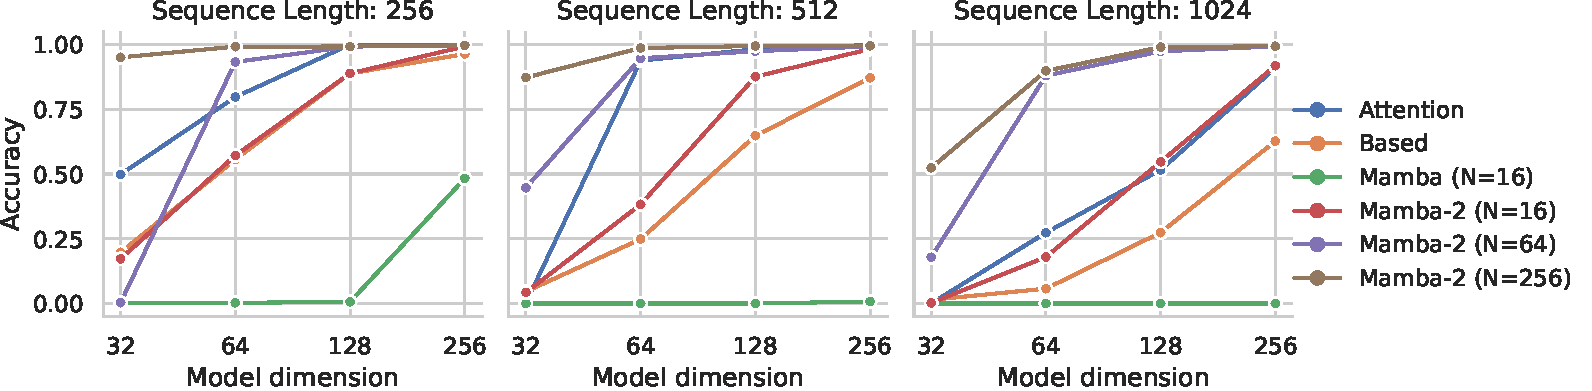
\includegraphics[width=\linewidth]{fig/mqar.pdf}
  \caption{
    (\textbf{Multi-Query Associative Recall (MQAR)}).
    Associative recall tasks are challenging for SSMs, which must memorize all relevant information into their recurrent state.
    The SSD layer combined with improved architecture allows for much larger state sizes in Mamba-2,
    which performs significantly better than Mamba-1 and even vanilla attention.
  }
  \label{fig:mqar}
\end{figure*}

\begin{figure}[!t]
  \centering
    \centering
    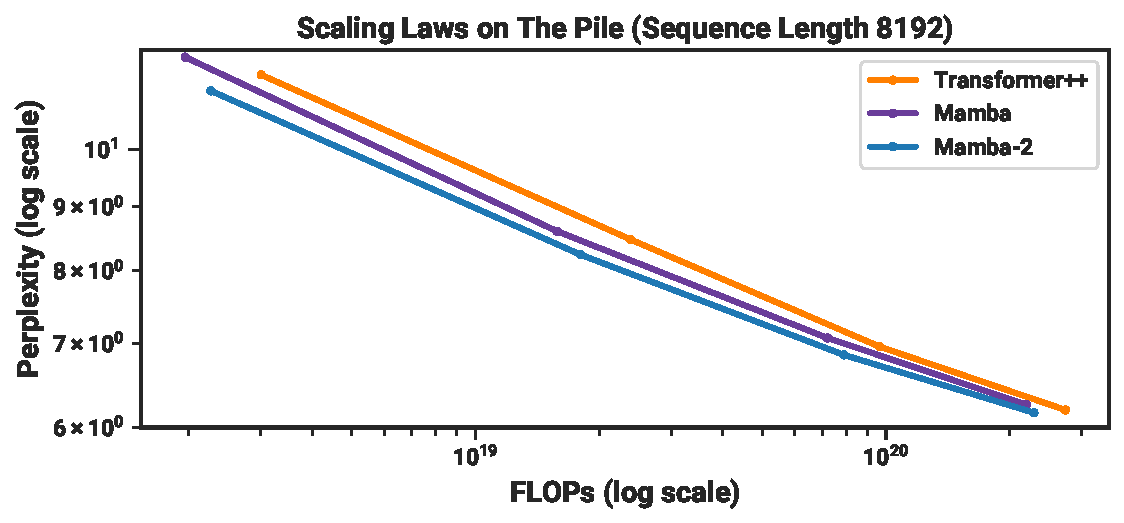
\includegraphics[width=\iftoggle{arxiv}{0.7\linewidth}{\linewidth}]{fig/pile_8k_mamba2.pdf}
  \caption{
    (\textbf{Scaling Laws}.) %
    Models of size $\approx 125M$ to $\approx 1.3B$ parameters, trained on the Pile.
    Mamba-2 matches or exceeds the performance of Mamba as well as a strong ``Transformer++'' recipe.
    Compared to our Transformer baseline, Mamba-2 is Pareto dominant on performance (perplexity), theoretical FLOPs, and actual wall-clock time.
  }
  \label{fig:lm-scaling}
  \iftoggle{arxiv}{}{\vspace{-1em}}
\end{figure}

\begin{table*}[!ht]
  \small
  \centering
  \captionsetup{font=small}
  \caption{
    (\textbf{Zero-shot Evaluations}.) Best results for each size in bold, second best unlined.
    We compare against open source LMs with various tokenizers, trained for up to 300B tokens.
    Pile refers to the validation split, comparing only against models trained on the same dataset and tokenizer (GPT-NeoX-20B).
    For each model size, Mamba-2 outperforms Mamba, and generally matches Pythia at twice the model size.
    Full results in \cref{table:downstream_zeroshot_full}.
  }
  \resizebox{0.99\linewidth}{!}
  {
    \begin{tabular}{@{}llllllllllll@{}}
      \toprule
      \sc{Model}                     & \sc{Token.} & \sc{Pile}          & \sc{LAMBADA}       & \sc{LAMBADA}       & \sc{HellaSwag}     & \sc{PIQA}          & \sc{Arc-E}         & \sc{Arc-C}           & \sc{WinoGrande}    & \sc{OpenbookQA}      & \sc{Average} \\
                                     &             & \sc{ppl $\downarrow$}       & \sc{ppl $\downarrow$}       & \sc{acc $\uparrow$}       & \sc{acc $\uparrow$}       & \sc{acc $\uparrow$}       & \sc{acc $\uparrow$}       & \sc{acc $\uparrow$}         & \sc{acc $\uparrow$}       & \sc{acc $\uparrow$}         & \sc{acc $\uparrow$} \\
                                        \midrule
      Pythia-1B                      & NeoX        & $7.82$             & $7.92$             & $56.1$             & $47.2$             & $70.7$             & $57.0$             & $27.1$               & $53.5$             & $31.4$               & $49.0$ \\
      Mamba-790M                     & NeoX        & $\underline{7.33}$ & $\underline{6.02}$ & $\mathbf{62.7}$    & $\mathbf{55.1}$    & $\mathbf{72.1}$    & $\mathbf{61.2}$    & $\mathbf{29.5}$      & $\underline{56.1}$ & $\underline{34.2}$   & $\underline{53.0}$ \\
      \textbf{Mamba-2-780M}          & NeoX        & $\mathbf{7.26}$    & $\mathbf{5.86}$    & $\underline{61.7}$ & $\underline{54.9}$ & $\underline{72.0}$ & $\underline{61.0}$ & $\underline{28.5}$   & $\mathbf{60.2}$    & $\mathbf{36.2}$      & $\mathbf{53.5}$ \\
      \midrule
      Hybrid H3-1.3B                 & GPT2        & ---                  & $11.25$            & $49.6$             & $52.6$             & $71.3$             & $59.2$             & $28.1$               & $56.9$             & $34.4$               & $50.3$ \\
      Pythia-1.4B                    & NeoX        & $7.51$             & $6.08$             & $61.7$             & $52.1$             & $71.0$             & $60.5$             & $28.5$               & $57.2$             & $30.8$               & $51.7$ \\
      RWKV4-1.5B                     & NeoX        & $7.70$             & $7.04$             & $56.4$             & $52.5$             & $72.4$             & $60.5$             & $29.4$               & $54.6$             & $34.0$               & $51.4$ \\
      Mamba-1.4B                     & NeoX        & $\underline{6.80}$ & $\underline{5.04}$ & $\underline{65.0}$ & $\underline{59.1}$ & $\mathbf{74.2}$    & $\mathbf{65.5}$    & $$\underline{32.8}$$ & $\mathbf{61.5}$    & $$\underline{36.4}$$ & $\mathbf{56.4}$ \\
      \textbf{Mamba-2-1.3B}          & NeoX        & $\mathbf{6.66}$    & $\mathbf{5.02}$    & $\mathbf{65.7}$    & $\mathbf{59.9}$    & $\underline{73.2}$ & $\underline{64.3}$ & $\mathbf{33.3}$      & $\underline{60.9}$ & $\mathbf{37.8}$      & $\mathbf{56.4}$ \\
      \midrule
      Hybrid H3-2.7B                 & GPT2        & ---                  & $7.92$             & $55.7$             & $59.7$             & $73.3$             & $65.6$             & $32.3$               & $61.4$             & $33.6$               & $54.5$ \\
      Pythia-2.8B                    & NeoX        & $6.73$             & $5.04$             & $64.7$             & $59.3$             & $74.0$             & $64.1$             & $32.9$               & $59.7$             & $35.2$               & $55.7$ \\
      RWKV4-3B                       & NeoX        & $7.00$             & $5.24$             & $63.9$             & $59.6$             & $73.7$             & $67.8$             & $33.1$               & $59.6$             & $37.0$               & $56.4$ \\
      Mamba-2.8B                     & NeoX        & $\underline{6.22}$ & $\underline{4.23}$ & $\underline{69.2}$ & $\underline{66.1}$ & $\underline{75.2}$ & $\mathbf{69.7}$    & $\underline{36.3}$   & $\underline{63.5}$ & $\mathbf{39.6}$      & $\underline{59.9}$ \\
      \textbf{Mamba-2-2.7B}          & NeoX        & $\mathbf{6.09}$    & $\mathbf{4.10}$    & $\mathbf{69.7}$    & $\mathbf{66.6}$    & $\mathbf{76.4}$    & $\underline{69.6}$ & $\mathbf{36.4}$      & $\mathbf{64.0}$    & $\underline{38.8}$   & $\mathbf{60.2}$ \\
      \bottomrule
    \end{tabular}
  }
  \label{table:downstream_zeroshot}
\end{table*}



\begin{figure*}[!ht]
  \centering
  \begin{subfigure}{.5\textwidth}
    \centering
    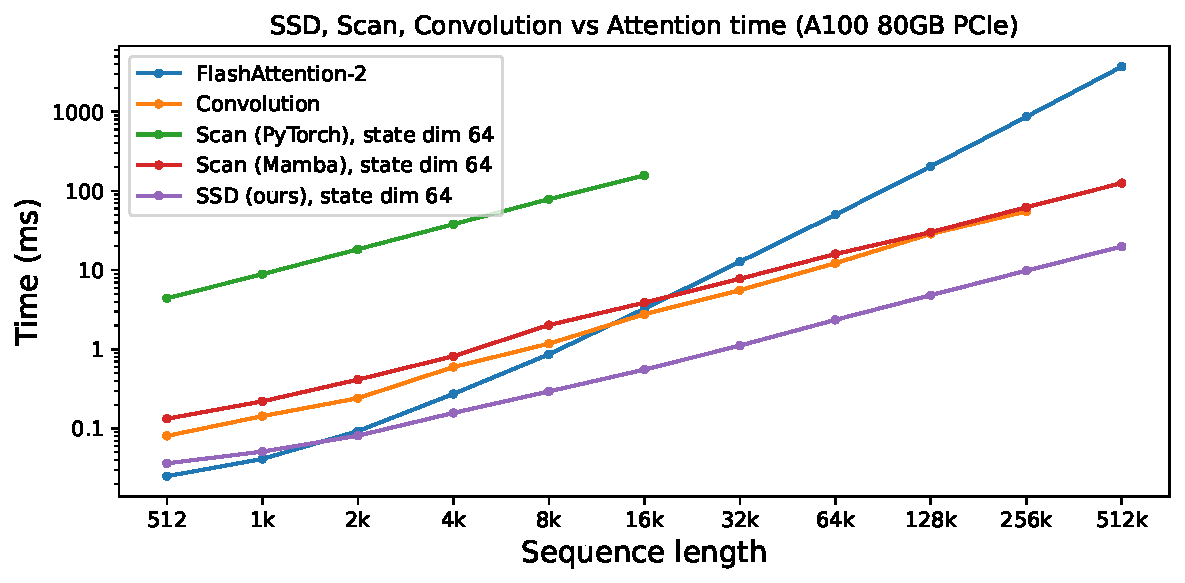
\includegraphics[width=.95\linewidth]{fig/ssm_ssd.pdf}
  \end{subfigure}%
  \begin{subfigure}{.5\textwidth}
    \centering
    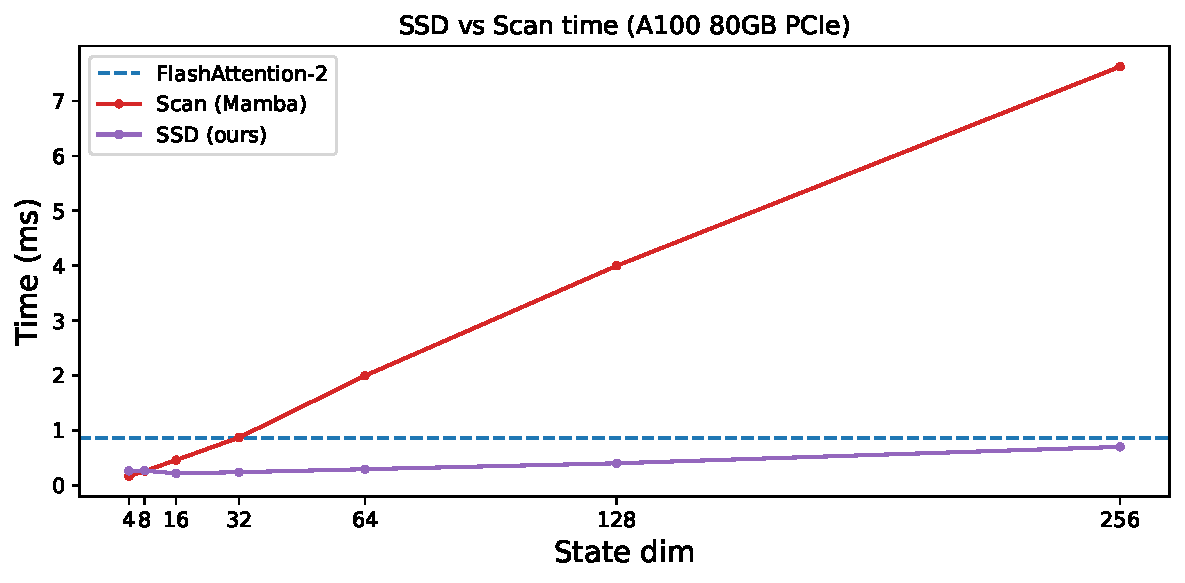
\includegraphics[width=.95\linewidth]{fig/ssm_ssd_dstate.pdf}
  \end{subfigure}
  \caption{
    (\textbf{Efficiency Benchmarks}.)
    (\emph{Left}) Our SSD is $2-8\times$ faster than a Mamba fused scan for large state expansion ($N = 64$) and faster than FlashAttention-2 for sequence length 2k and above.
    (\emph{Right}) Sequence length 4K: Increasing state expansion slows down the Mamba optimized scan implementation linearly. SSD can handle much larger state expansion factors without much slowdown.
    \iftoggle{arxiv}{}{\vspace*{-0.75em}}
  }
  \label{fig:scan_benchmark}
\end{figure*}



\subsection{Synthetics: Associative Recall}
\label{sec:experiments:mqar}

Synthetic associative recall tasks have been popular for testing the ability of language models to look up information in their context.
Broadly, they involve feeding autoregressive models pairs of key-value associations, and then prompting the model to produce the correct completion upon being shown a previously-seen key.
The \textbf{multi-query associative recall (MQAR)} task is a particular formulation of this task that requires the model to memorize multiple associations~\citep{arora2024zoology}.
\iftoggle{arxiv}{
The original Mamba paper reported results on related synthetic tasks, in particular Selective Copying~\citep{gu2023mamba} and Induction Heads~\citep{olsson2022context}, which can be seen as easier associative recall tasks.
The MQAR task is also closely related to ``phonebook look-up'' tasks which has been shown to be challenging for recurrent models such as SSMs, due to their finite state capacity~\citep{jelassi2024repeat,de2024griffin}.
}{}

We compare on a challenging version of the MQAR setup from~\citep{arora2024simple}, using a harder task, longer sequences, and smaller models.
Our baselines include standard multi-head softmax attention as well as the Based architecture which combines convolutions, local attention, and a linear attention variant.

Results are shown in \cref{fig:mqar}.
While Mamba-1 struggles on this task, Mamba-2 performs well across all settings.
\iftoggle{arxiv}{
Surprisingly, it is significantly better than Mamba-1 even when the state sizes are controlled ($\mathtt{N}=16$).
(We are not sure which aspect of the architecture is the predominant factor, which remains a question to explore in future work.)
Additionally, this task validates the importance of state size: increasing from $\mathtt{N}=16$ to $\mathtt{N}=64$ and $\mathtt{N}=256$ consistently improves performance on MQAR, as the larger state allows more information (key-value pairs) to be memorized.
}{}

\subsection{Language Modeling}
\label{sec:experiments:lm}

Following standard protocols in LLMs, we train and evaluate the Mamba-2 architecture on standard autoregressive language modeling against other architectures.
We compare both pretraining metrics (perplexity) and zero-shot evaluations.
The model sizes (depth and width) follow GPT3 specifications, from 125m to 2.7B. %
We use the Pile dataset~\citep{pile}, and follow the training recipe described in~\citet{brown2020language}.
This follows the same setup as reported in Mamba~\citep{gu2023mamba};
training details are in~\cref{sec:exp-details}.

\subsubsection{Scaling Laws}
For baselines, we compare against both Mamba and its Transformer++ recipe~\citep{gu2023mamba}, which is based on the PaLM and LLaMa architectures (e.g.\ rotary embedding, SwiGLU MLP, \iftoggle{arxiv}{RMSNorm instead of LayerNorm, no linear bias, and higher learning rates}{etc.}).
As Mamba has already demonstrated that it outperforms the standard Transformer architecture (GPT3 architecture) as well as recent subquadratic architectures (H3~\citep{dao2023hungry}, Hyena~\citep{poli2023hyena}, RWKV-4~\citep{peng2023rwkv}, RetNet~\citep{sun2023retentive}), we omit those in the plot for clarity (see \citet{gu2023mamba} for comparisons).

\iftoggle{arxiv}{
\cref{fig:lm-scaling} shows scaling laws under the standard Chinchilla~\citep{hoffmann2022empirical} protocol,
on models from $\approx 125M$ to $\approx 1.3B$ parameters.

}{}


\subsubsection{Downstream Evaluations}

\cref{table:downstream_zeroshot} shows the performance of Mamba-2 on a range of popular downstream zero-shot evaluation tasks, compared to the most well-known open source models at these sizes,
most importantly Pythia~\citep{biderman2023pythia} which were trained with the same tokenizer, dataset, and training length (300B tokens) as our models.



\subsubsection{Hybrid Models: Combining SSD Layer with MLP and Attention}
\label{sec:hybrid}

Recent and concurrent work~\citep{dao2023hungry,de2024griffin,lieber2024jamba,glorioso2024zamba} suggests that a hybrid architecture with both SSM layers and
attention layers could improve the model quality over that of a Transformer, or a
pure SSM (e.g., Mamba) model, especially for in-context learning.
We explore the different ways that SSD layers can be combined with attention and
MLP to understand the benefits of each.
Empirically we find that having around 10\% of the total
number of layers being attention performs best.
Combining SSD layers, attention layers, and MLP also works better than either
pure Transformer++ or Mamba-2.

\paragraph{SSD and Attention}
We find that SSD and attention layers are complementary: by themselves (e.g.
in the Mamba-2 architecture vs. Transformer++) their performance (measured by
perplexity) is nearly the same, but a mixture of SSD and attention layers
outperforms the pure Mamba-2 or Transformer++ architecture. We show some results
(\cref{tab:ssd_attn}) for the 350M model (48 layers) trained to 7B tokens on the Pile with the GPT-2 tokenizer (same
number of parameters, same hyperparameters, same training and validation set).
Adding in just a few attention layers already yields notable improvement and
strikes the best balance between quality and efficiency. We hypothesize that
the SSM layers function well as a general sequence-to-sequence mapping, and
attention layers act as a retrieval mechanism to quickly refer to previous
tokens in the sequence instead of forcing the model to compress all the context
to its memory (SSM states).

\begin{table*}[ht]
  \small
  \caption{
    (\textbf{Combining SSD and Attention Blocks}.) Perplexity of a 350M model
    with 48 layers, with different number of attention layers.
    Having around a 10\% ratio of attention layers performs best.
  }
  \centering
  \begin{tabular}{@{}llllllllllllll@{}}
    \toprule
    \sc{Num.\ Attn Blocks} & 0 (Mamba-2) & 1 & 2 & 3 & 4 & 5 & 6 & 7 & 9 & 11 & 15 & 24 & Transformer++ \\
    \midrule
    \sc{Perplexity} $\downarrow$ & 8.60 & 8.38 & 8.32 & 8.29 & 8.29 & 8.28 & \textbf{8.26} & 8.27 & 8.28 & 8.30 & 8.34 & 8.50 & 8.68\\
    \bottomrule
  \end{tabular}
  \label{tab:ssd_attn}
\end{table*}

\paragraph{Hybrid Models with SSD, MLP, and Attention}

We compare different ways that SSD can be combined with the (gated) MLP and attention layers, and evaluate at the 2.7B scale (64 layers), trained to 300B tokens on the Pile (same
number of parameters, same hyperparameters, same training and validation set, same data order):
\begin{enumerate}
\item Transformer++: 32 attention layers and 32 gated MLP, interleaving.
\item Mamba-2: 64 SSD layers.
\item Mamba-2-MLP: 32 SSD and 32 gated MLP layers, interleaving.
\item Mamba-2-Attention: 58 SSD layers and 6 attention layers (at indices 9, 18, 27, 36, 45, 56)\footnote{In small-scale experiments, we find that as long as the attention layers are spaced out, not at the very beginning or at the very end, the model quality does not depend very much on the exact location of the attention layers.}.
\item Mamba-2-MLP-Attention: 28 SSD layers and 4 attention layers, interleaving with 32 gated MLP layers.
\end{enumerate}
We report the validation perplexity on the Pile, as well as zero-shot evaluation, in~\cref{table:hybrid_eval}.
In general, the quality of Transformer++ and Mamba-2 models are around the same.
We see that adding just 6 attention layers noticeably improves over the pure Mamba-2 model (and over Transformer++). Adding MLP layers reduces model quality, but can (i) speed up training and inference due to the simplicity and hardware-efficiency of the MLP layer (ii) be easier to up-cycle to MoE models by replacing MLP layers with mixture-of-experts.
\begin{table*}[!ht]
  \centering
  \captionsetup{font=small}
  \caption{
    (\textbf{Zero-shot Evaluations}.) Best results for each size in bold.
    We compare different ways SSD, MLP, and attention layers can be combined, evaluated at 2.7B scale trained to 300B tokens on the Pile.
  }
  \resizebox{0.99\linewidth}{!}
  {
    \begin{tabular}{@{}llllllllllll@{}}
      \toprule
      \sc{Model}                  & \sc{Token.} & \sc{Pile}             & \sc{LAMBADA}          & \sc{LAMBADA}        & \sc{HellaSwag}      & \sc{PIQA}           & \sc{Arc-E}          & \sc{Arc-C}          & \sc{WinoGrande}     & \sc{OpenbookQA}     & \sc{Average} \\
                                  &             & \sc{ppl $\downarrow$} & \sc{ppl $\downarrow$} & \sc{acc $\uparrow$} & \sc{acc $\uparrow$} & \sc{acc $\uparrow$} & \sc{acc $\uparrow$} & \sc{acc $\uparrow$} & \sc{acc $\uparrow$} & \sc{acc $\uparrow$} & \sc{acc $\uparrow$} \\
      \midrule
      Transformer++               & NeoX        & 6.13                  & 3.99                  & \underline{70.3}    & 66.4                & 75.2                & 67.7                & \underline{37.8}    & 63.9                & \textbf{40.4}       & 60.2 \\
      Mamba-2                     & NeoX        & 6.09                  & 4.10                  & 69.7                & \underline{66.6}    & \textbf{76.4}       & 69.6                & 36.4                & 64.0                & 38.8                & 60.2 \\
      Mamba-2-MLP                 & NeoX        & 6.13                  & 4.18                  & 69.3                & 65.0                & \textbf{76.4}       & 68.1                & 37.0                & 63.1                & 38.2                & 59.6 \\
      Mamba-2-Attention           & NeoX        & \textbf{5.95}         & \textbf{3.85}         & \textbf{71.1}       & \textbf{67.8}       & \underline{75.8}    & \underline{69.9}    & \underline{37.8}    & \textbf{65.3}       & 39.0                & \textbf{61.0} \\
      Mamba-2-MLP-Attention       & NeoX        & \underline{6.00}      & \underline{3.95}      & 70.0                & \underline{66.6}    & 75.4                & \textbf{70.6}       & \textbf{38.6}       & \underline{64.6}    & \underline{39.2}    & \underline{60.7} \\
      \bottomrule
    \end{tabular}
  }
  \label{table:hybrid_eval}
\end{table*}

\subsection{Speed Benchmarks}
\label{sec:experiments:benchmark}

We benchmark the speed of the SSD algorithm against Mamba's scan implementation and FlashAttention-2 (\cref{fig:scan_benchmark}).
SSD, thanks to its reformulation to use matrix multiplication as a subroutine, can exploit specialized matrix multiplication (matmul) units on GPUs, also known as tensor cores.
As a result, it is 2-8$\times$ faster than Mamba's fused associative scan, which does not leverage matmul units.
Due to its linear scaling in sequence length, SSD is faster than FlashAttention-2 starting at sequence length $2K$.

However, we note that the Mamba-2 model as a whole might not be as efficient to train as Transformer at short sequence length (e.g. at $2K$), since a Transformer with $L$ layers would have $\frac{L}{2}$ MLP layers and $\frac{L}{2}$ attention layers, while a Mamba-2 model would have $L$ SSD layers for the same number of parameters.
Generally the MLP layers are very hardware efficient since they consist of simple matrix multiplication and pointwise linearity.
As shown in~\cref{sec:hybrid}, one can also combine $\frac{L}{2}$ SSD layers and $\frac{L}{2}$ MLP layers to speed up training at short sequence length.

\iftoggle{arxiv}{
\subsection{Architecture Ablations}
\label{sec:experiments:ablations}

\subsubsection{Block Design}
\label{sec:experiments:ablations:block}

\cref{sec:architecture:block} introduces the Mamba-2 block, which has small modifications to the Mamba-1 block which are partly motivated by the connection to attention and also to improve the scalability of Mamba-2.
\cref{tab:ablations-architecture} ablates these architecture changes to the block, which occur outside of the core SSM layer.

The ablations validate that parallel projections to create $(A,B,C,X)$ saves parameters and performs slightly better than Mamba's sequential projections.
More importantly, this modification is amenable to tensor parallelism at larger model sizes (\cref{sec:systems}).
Additionally, the extra normalization layer also slightly improves performance.
More importantly, preliminary experiments at larger scales observed that it also helps with training stability.

\begin{table}
  \caption{
    (\textbf{Ablations: Mamba-2 block}.)
    We ablate the major differences between the Mamba-2 and Mamba-1 neural network blocks (\cref{fig:architecture}, \cref{sec:architecture:block}).
    Note that these components are independent of the inner sequence mixing layer; in these ablations, we use SSD for the inner SSM layer (differing from the S6 layer of Mamba-1).
  }
  \centering
  \begin{tabular}{@{}lllll@{}}
    \toprule
    Block & $ABCX$ \sc{Projections} & \sc{Extra Normalization} & \sc{Parameters} & \sc{Perplexity} \\
    \midrule
    Mamba-1 & Sequential              & \xmark                   & 129.3M          & 11.76 \\
            & Sequential              & \cmark                   & 129.3M          & 11.54 \\
            & Parallel                & \xmark                   & 126.5M          & 11.66 \\
    Mamba-2 & Parallel                & \cmark                   & 126.5M          & 11.49 \\
    \bottomrule
  \end{tabular}
  \label{tab:ablations-architecture}
\end{table}

\subsubsection{Head Structure}

\cref{sec:architecture:multihead} describes how the dimensions of the $B, C, X$ projections can be viewed as a hyperparameter analogous to notions of multi-head attention and multi-query attention.
We also showed how the original Mamba architecture is analogous to multi-value attention (\cref{prop:mamba-multihead}),
which was a choice that naturally developed from the state-space model point of view and was not previously ablated.

\cref{tab:ablations-heads} ablates choices of the multi-head structure for the Mamba-2 architecture.
Strikingly, we find a large difference between multi-value and multi-query or multi-key head patterns,
despite seeming very similar.
Note that this is not explained by the total state size, which is the same for all of them (equal to $\mathtt{HPN}$ or the product of the number of heads, head dimension, and state dimension).

We also compare to multi-head patterns where the number of $C, B, X$ (analogous to $Q, K, V$) heads is equal.
We compare against the standard multi-head pattern, as well as one with aggressive sharing where they all have only $1$ head.
Note that in the latter case, the model still has $\mathtt{H}$ different sequence mixers $M$, because each head still has a different $A$.
When parameter matched, these multi-head patterns perform similarly to each other, in between the MVA and MQA/MKA patterns.

\begin{table}[!th]
  \small
  \centering
  \captionsetup{type=table}
  \caption{
    (\textbf{Ablations: Multi-head structure}.)
    All models have state expansion factor $N=64$ and head size $P=64$ and are trained to Chinchilla scaling law token counts.
    The number of $A$ heads is always equal to the total heads $\mathtt{H}$, i.e. each head has a separate input-dependent $A$ decay factor.
    (\emph{Top}) 125M models, 2.5B tokens
    (\emph{Bottom}) 360M models, 7B tokens
  }
  \begin{tabular}{@{}lllllllll@{}}
    \toprule
    \sc{SSM Head Pattern} & \sc{Attn. Analog} & $A$ \sc{heads} & $B$ \sc{heads} & $C$ \sc{heads} & $X$ \sc{heads} & \sc{Layers} & \sc{Params} & \sc{Ppl.} \\
    \midrule
    Multi-input (MIS)     & Multi-value (MVA) & 24             & 1              & 1              & 24             & 24          & 126.5M      & $\mathbf{11.66}$ \\
    Multi-contract (MCS)  & Multi-query (MQA) & 24             & 1              & 24             & 1              & 24          & 126.5M      & $12.62$ \\
    Multi-expand (MES)    & Multi-key (MKA)   & 24             & 24             & 1              & 1              & 24          & 126.5M      & $12.59$ \\
    Multi-head (MHS)      & Multi-head (MHA)  & 24             & 24             & 24             & 24             & 15          & 127.6M      & $12.06$ \\
    Multi-state (MSS)     & -                 & 24             & 1              & 1              & 1              & 36          & 129.6M      & $12.00$ \\
    \midrule
    Multi-input (MIS)     & Multi-value (MVA) & 32             & 1              & 1              & 32             & 48          & 361.8M      & $\mathbf{8.73}$ \\
    Multi-contract (MCS)  & Multi-query (MQA) & 32             & 1              & 32             & 1              & 48          & 361.8M      & $9.33$ \\
    Multi-expand (MES)    & Multi-key (MKA)   & 32             & 32             & 1              & 1              & 48          & 361.8M      & $9.36$ \\
    Multi-head (MHS)      & Multi-head (MHA)  & 32             & 1              & 1              & 1              & 70          & 361.3M      & $9.01$ \\
    Multi-state (MSS)     & -         & 32             & 32             & 32             & 32             & 29          & 357.3M      & $9.04$ \\
    \bottomrule
  \end{tabular}
  \label{tab:ablations-heads}
\end{table}

\subsubsection{Attention Kernel Approximations}
\label{sec:experiments:ablations:kernels}


\cref{sec:architecture:kernels} noted how SSD can be combined with ideas from the linear attention literature,
such as various forms of kernel approximations.
We ablate several variants of these suggested by previous works in \cref{tab:ablations-kernel}.
These include the cosFormer~\citep{qin2022cosformer}, Random Feature Attention~\cite{peng2021random}, and Positive Random Features (Performer)~\citep{choromanski2021rethinking}.

We also ablate adding a normalization term, akin to the denominator of the softmax function in standard attention.
We found that this introduced instabilities to most variants, but slightly improved performance for the ReLU activation function $\psi$.

\cref{tab:ablations-kernel-based} also tests more recent proposals to improve linear attention that involve expanding the feature dimension (Based~\citep{arora2024simple} and ReBased~\citep{aksenov2024linear}).
These linear attention extensions aim to appropriate the $\exp$ kernel with a quadratic approximation.
ReBased also proposes to replace the QK activation function with a layer normalization;
from an SSM-centric view we apply a normalization on top of $(B, C)$ before applying the SSM function.
We note that this technique has been independently proposed as the ``QK-Norm'' for softmax attention~\citep{team2024chameleon}
and an ``internal normalization'' for Mamba~\citep{lieber2024jamba}.

Overall, \cref{tab:ablations-kernel} and \cref{tab:ablations-kernel-based} found that the kernel approximation methods we tried did not seem to improve over simple pointwise non-linear activation functions for $\psi$.
Thus our default settings for Mamba-2 used $\psi(x) = \mathsf{Swish}(x)$ to follow Mamba-1,
but we suggest that removing this activation entirely may be a simpler choice that we did not extensively test.

We emphasize however that SSD and vanilla linear attention differ in the inclusion of the 1-semiseparable mask $L$, while the various linear attention methods in the literature were derived to approximate softmax attention without this term; thus, our negative results may be not unexpected.

\begin{figure}[!t]
  \begin{minipage}{.5\linewidth}
    \centering
    \captionsetup{type=table}
    \caption{
      (\textbf{Ablations: Kernel approximations}.)
      We test various proposals for the kernel activation function $\psi$, including linear attention variants aiming to approximate the $\exp$ kernel from standard softmax attention.
    }
    \begin{tabular}{@{}llll@{}}
      \toprule
      \sc{Kernel activation $\varphi$} & \sc{Perplexity} \\
      \midrule
      none                             & $11.58$ \\
      Swish                            & $11.66$ \\
      Exp                              & $11.62$ \\
      ReLU                             & $11.73$ \\
      ReLU + normalization             & $11.64$ \\
      \midrule
      cosFormer                        & $11.97$ \\
      Random Feature Attention         & $11.57$ \\
      Positive Random Features (Performer) & $12.21$ \\
      \bottomrule
    \end{tabular}
    \label{tab:ablations-kernel}
  \end{minipage}
\hfill
\begin{minipage}{.45\linewidth}
  \centering
  \captionsetup{type=table}
  \caption{
    (\textbf{Ablations: Kernel approximations}.)
    We test the (Re)Based methods for linear attention approximations, which involve expanded feature maps.
    (\emph{Top}) 130M models. (\emph{Top}) 380M models with $N=256$.
  }
  \begin{tabular}{@{}lll@{}}
    \toprule
    \sc{Kernel activation $\varphi$} & \sc{Perplexity} \\
    \midrule
    Swish                            & $11.67$         \\
    Swish + Taylor (Based)           & $12.19$         \\
    LayerNorm                        & $11.50$         \\
    LayerNorm + Square (ReBased)     & $11.84$         \\
    \midrule
    Swish                            & $8.58$ \\
    Swish + Taylor (Based)           & $8.71$ \\
    LayerNorm                        & $8.61$ \\
    LayerNorm + Square (ReBased)     & $8.63$ \\
    \bottomrule
  \end{tabular}
  \label{tab:ablations-kernel-based}
\end{minipage}
\end{figure}
}{}
